To reject background events arising from the decay of a W boson, two variables are used, the transverse mass of the $\mu$+$\met$ system ($M_{T}$), and $\pzetadiff$.
To reject this background for the MSSM Higgs search, the kinematics of tau decays is leveraged in the use of $\pzetadiff$.
In di-tau signal events the neutrinos are expected to be nearly collinear with the associated visible decay products, thus the direction of the missing transverse energy would lie between the visible decay products.
In contrast, events in which a lepton is produced via a semi-leptonic W boson decay, and to a lesser extent $t\overline{t}$ events, this correlation does not exist.
An axis $\zeta$ is defined by bisecting the directions of the visible decay products, the momentum of the visible decay products is then projected onto this axis producing the observable $p_{\zeta}^{vis}$.
An additional observable $p_{\zeta}^{miss}$ is created by projecting the missing transverse energy vector onto the same bisecting axis $\zeta$.
A final observable $\pzetadiff$ is used to reject W background events, it is defined as:
\begin{equation}
\label{eqn:pzetadiff}
\pzetadiff = p_{\zeta}^{miss} -  1.5 p_{\zeta}^{vis}
\end{equation}

In the SM search, the Higgs decays will tend to have a softer $p_{T}$ spectrum leading to the decay products being less collimated.
For this reason in order to reject this background in SM Higgs search the transverse mass is used to discriminate against events which arise from the semi-leptonic decay of a W boson.
The transverse mass is defined as 
\begin{equation}
\label{eqn:mt}
   M_{T} = p_{T}^{\mu}\met\sqrt{1-cos\Delta\phi},
\end{equation}
where $\Delta\phi$ is the angle between the muon's momentum vector and the reconstructed $\met$.
The transverse mass is required to be less than $40$ GeV.
Both the transverse mass and $\pzetadiff$ distributions can be seen in Figure \ref{fig:mtpzeta}.

\begin{figure}[ht]
  \begin{minipage}[b]{0.5\linewidth}
\centering
  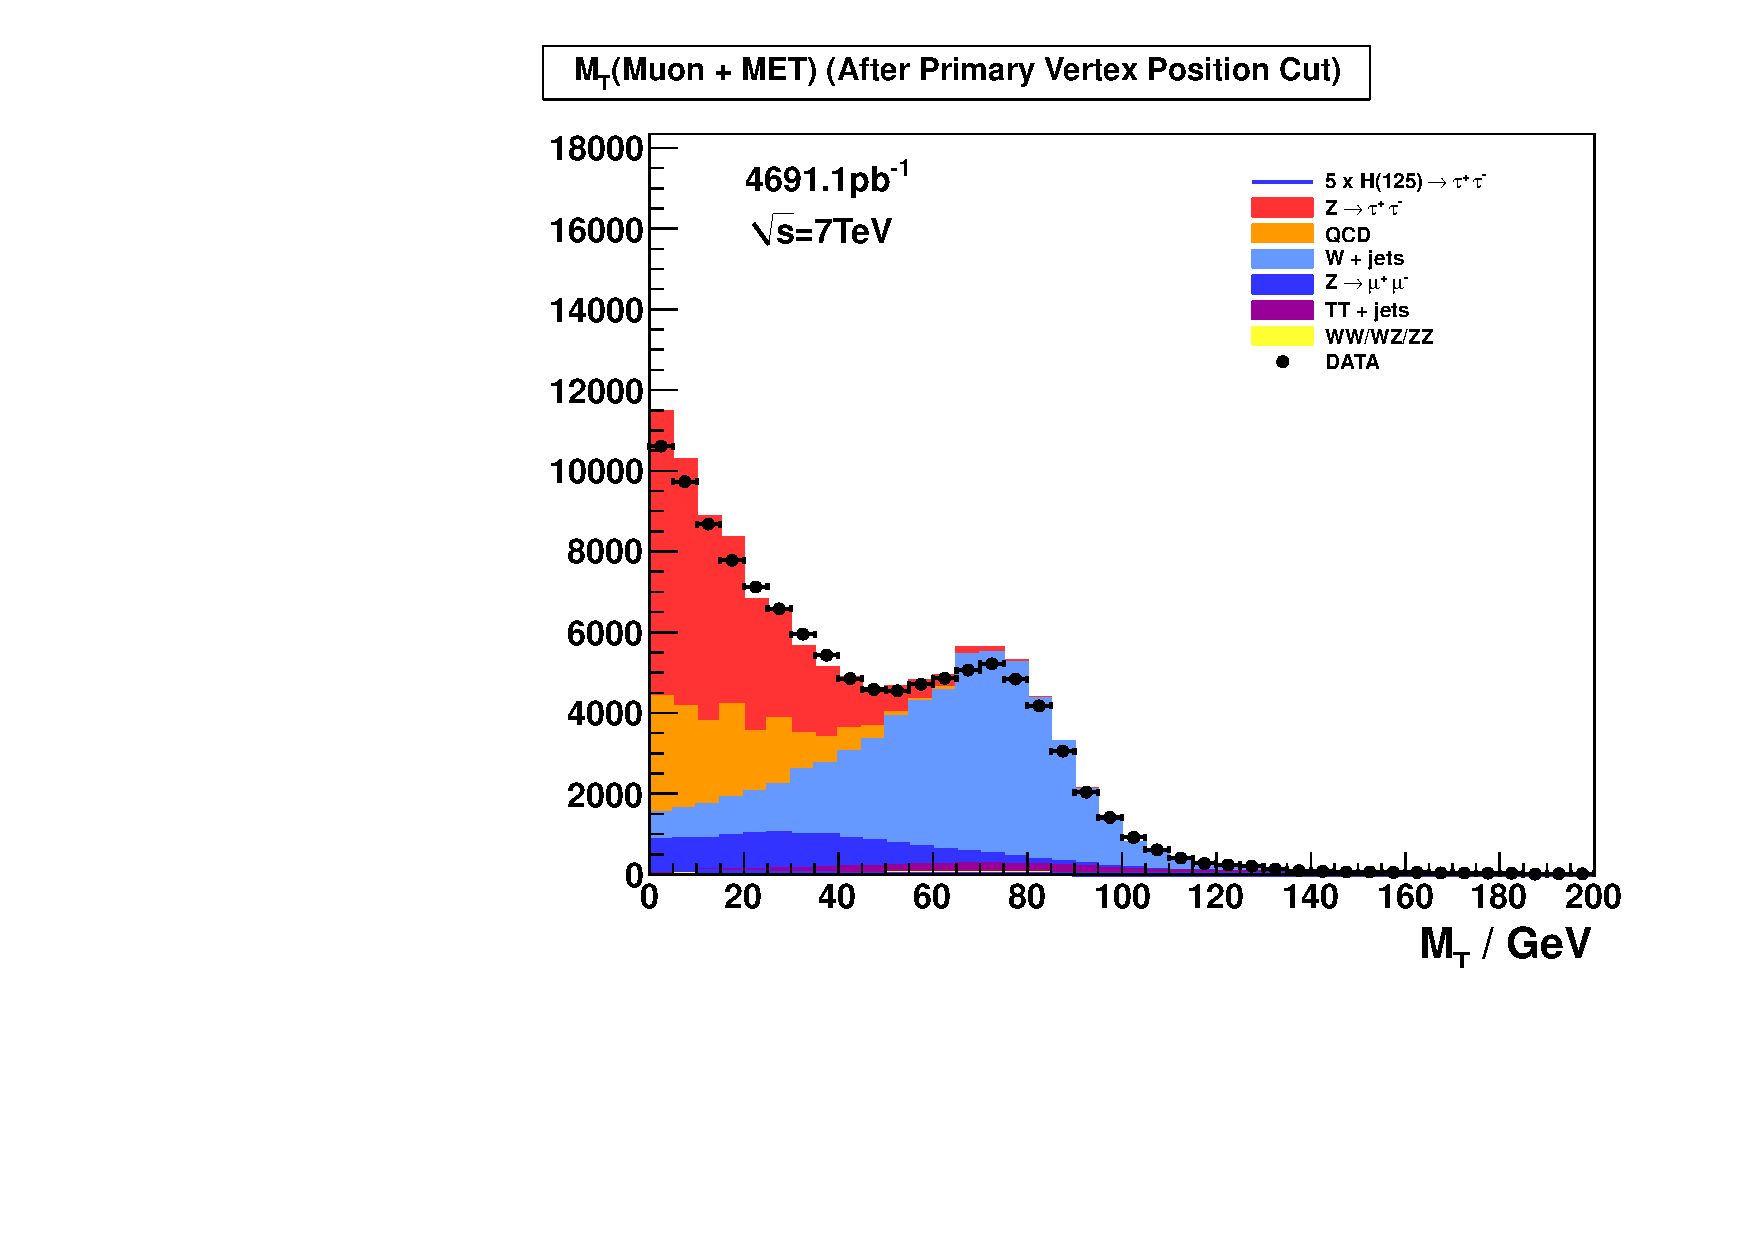
\includegraphics[scale=0.35]{plots/plotAHtoMuTau_leptonSelection_18_afterEvtSelPrimaryEventVertexPositionForMuTau_beforeEvtSelDiTauCandidateForMuTauMt1MET_mtMuonMET_linear.pdf}
\end{minipage}
\hspace{0.5cm}
\begin{minipage}[b]{0.5\linewidth}
\centering
  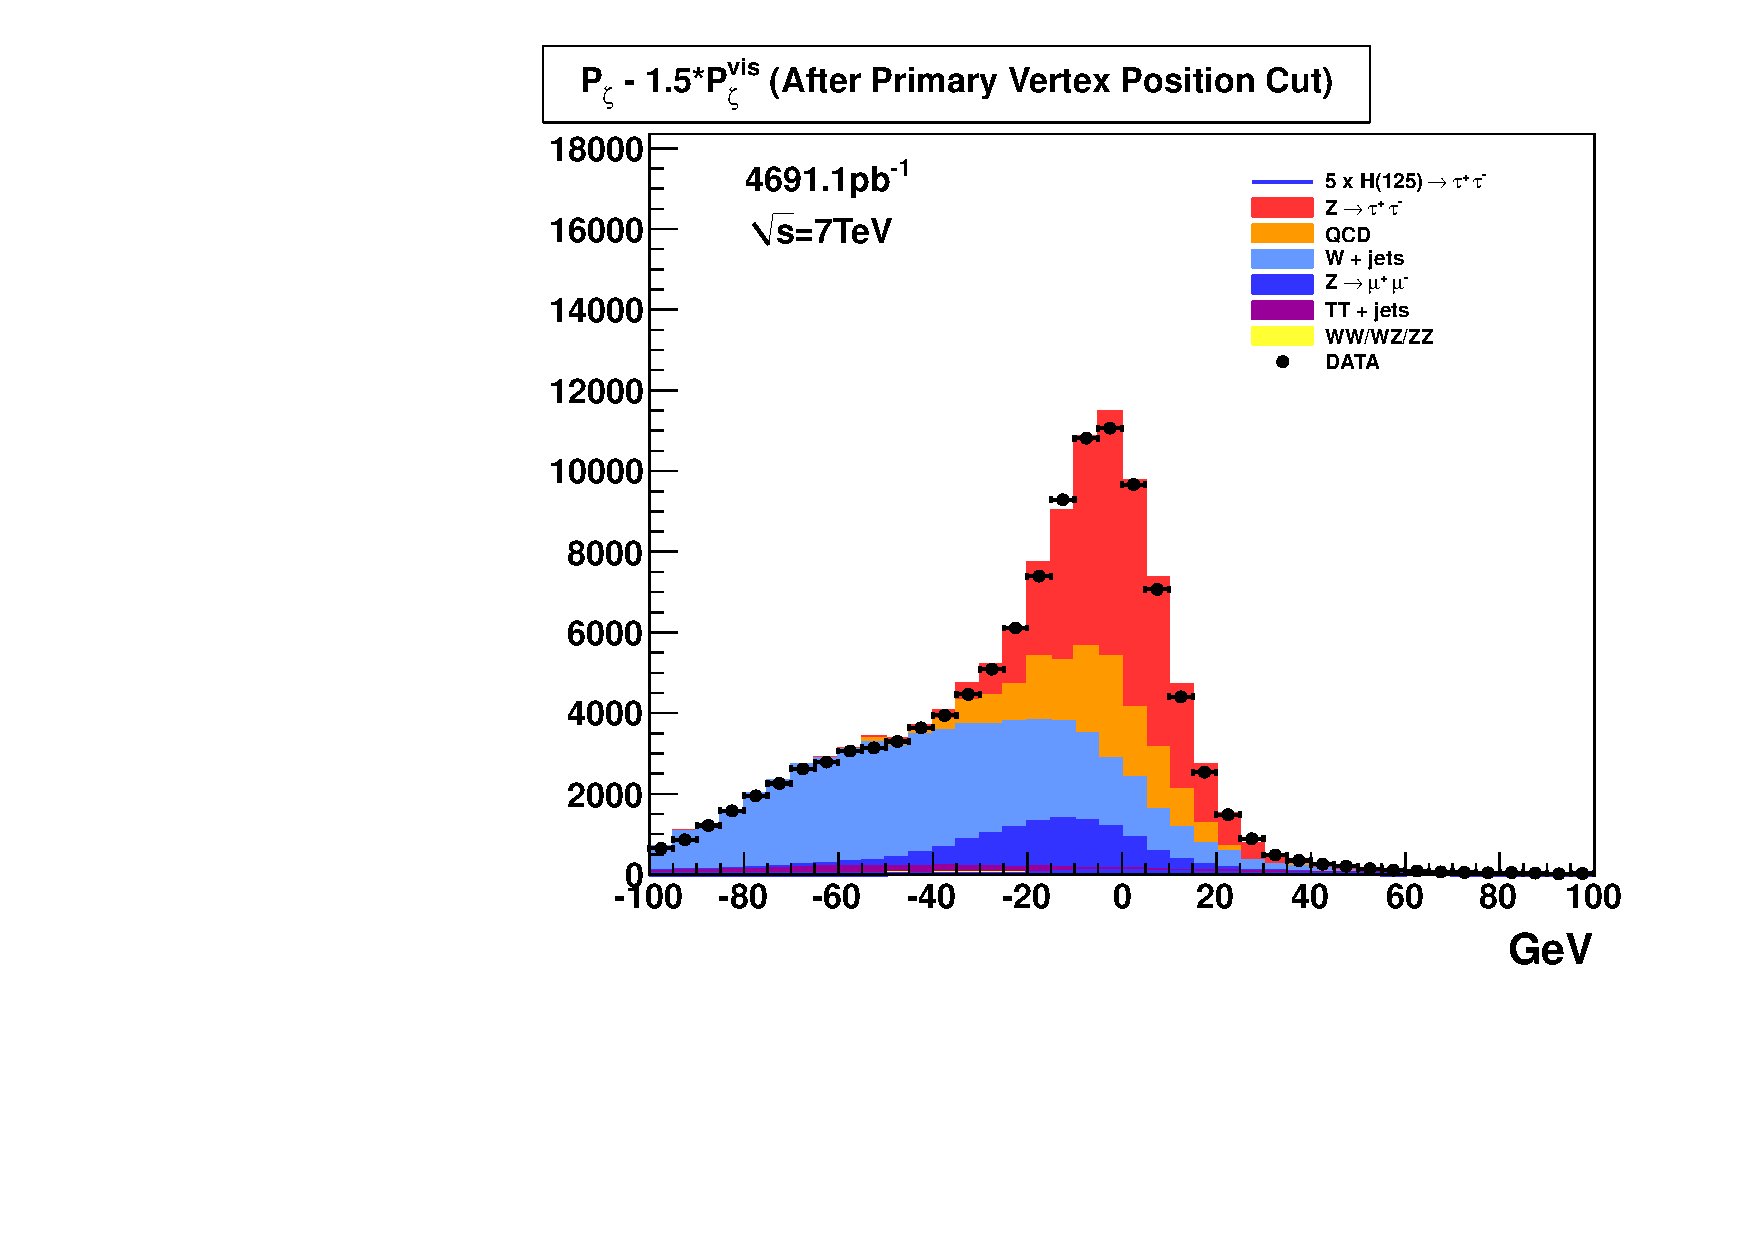
\includegraphics[scale=0.35]{plots/plotAHtoMuTau_leptonSelection_18_afterEvtSelPrimaryEventVertexPositionForMuTau_beforeEvtSelDiTauCandidateForMuTauMt1MET_PzetaDiff_linear}
\end{minipage}
\caption{$M_{T}$ and $\pzetadiff$ distributions.}
\label{fig:mtpzeta}
\end{figure}
